% Ring mit p Prozessoren
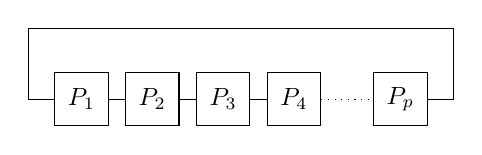
\begin{tikzpicture}
    [
        processor/.style={rectangle, draw, scale=0.9, minimum size=5ex},
        scale=0.9,
    ]
    \node (p1) at (1,0) [processor] {$P_1$};
    \node (p2) at (2,0) [processor] {$P_2$};
    \node (p3) at (3,0) [processor] {$P_3$};
    \node (p4) at (4,0) [processor] {$P_4$};
    \node (pp) at (5.5,0) [processor] {$P_p$};
    \draw (p1) -- (p2) -- (p3) -- (p4);
    \draw [dotted] (p4) -- (pp);
    \draw (pp) -- (6.25,0) -- (6.25,1) -- (0.25,1) -- (0.25,0) -- (p1);
\end{tikzpicture}         
